\begin{figure}\centering
	\subfloat[]{%
		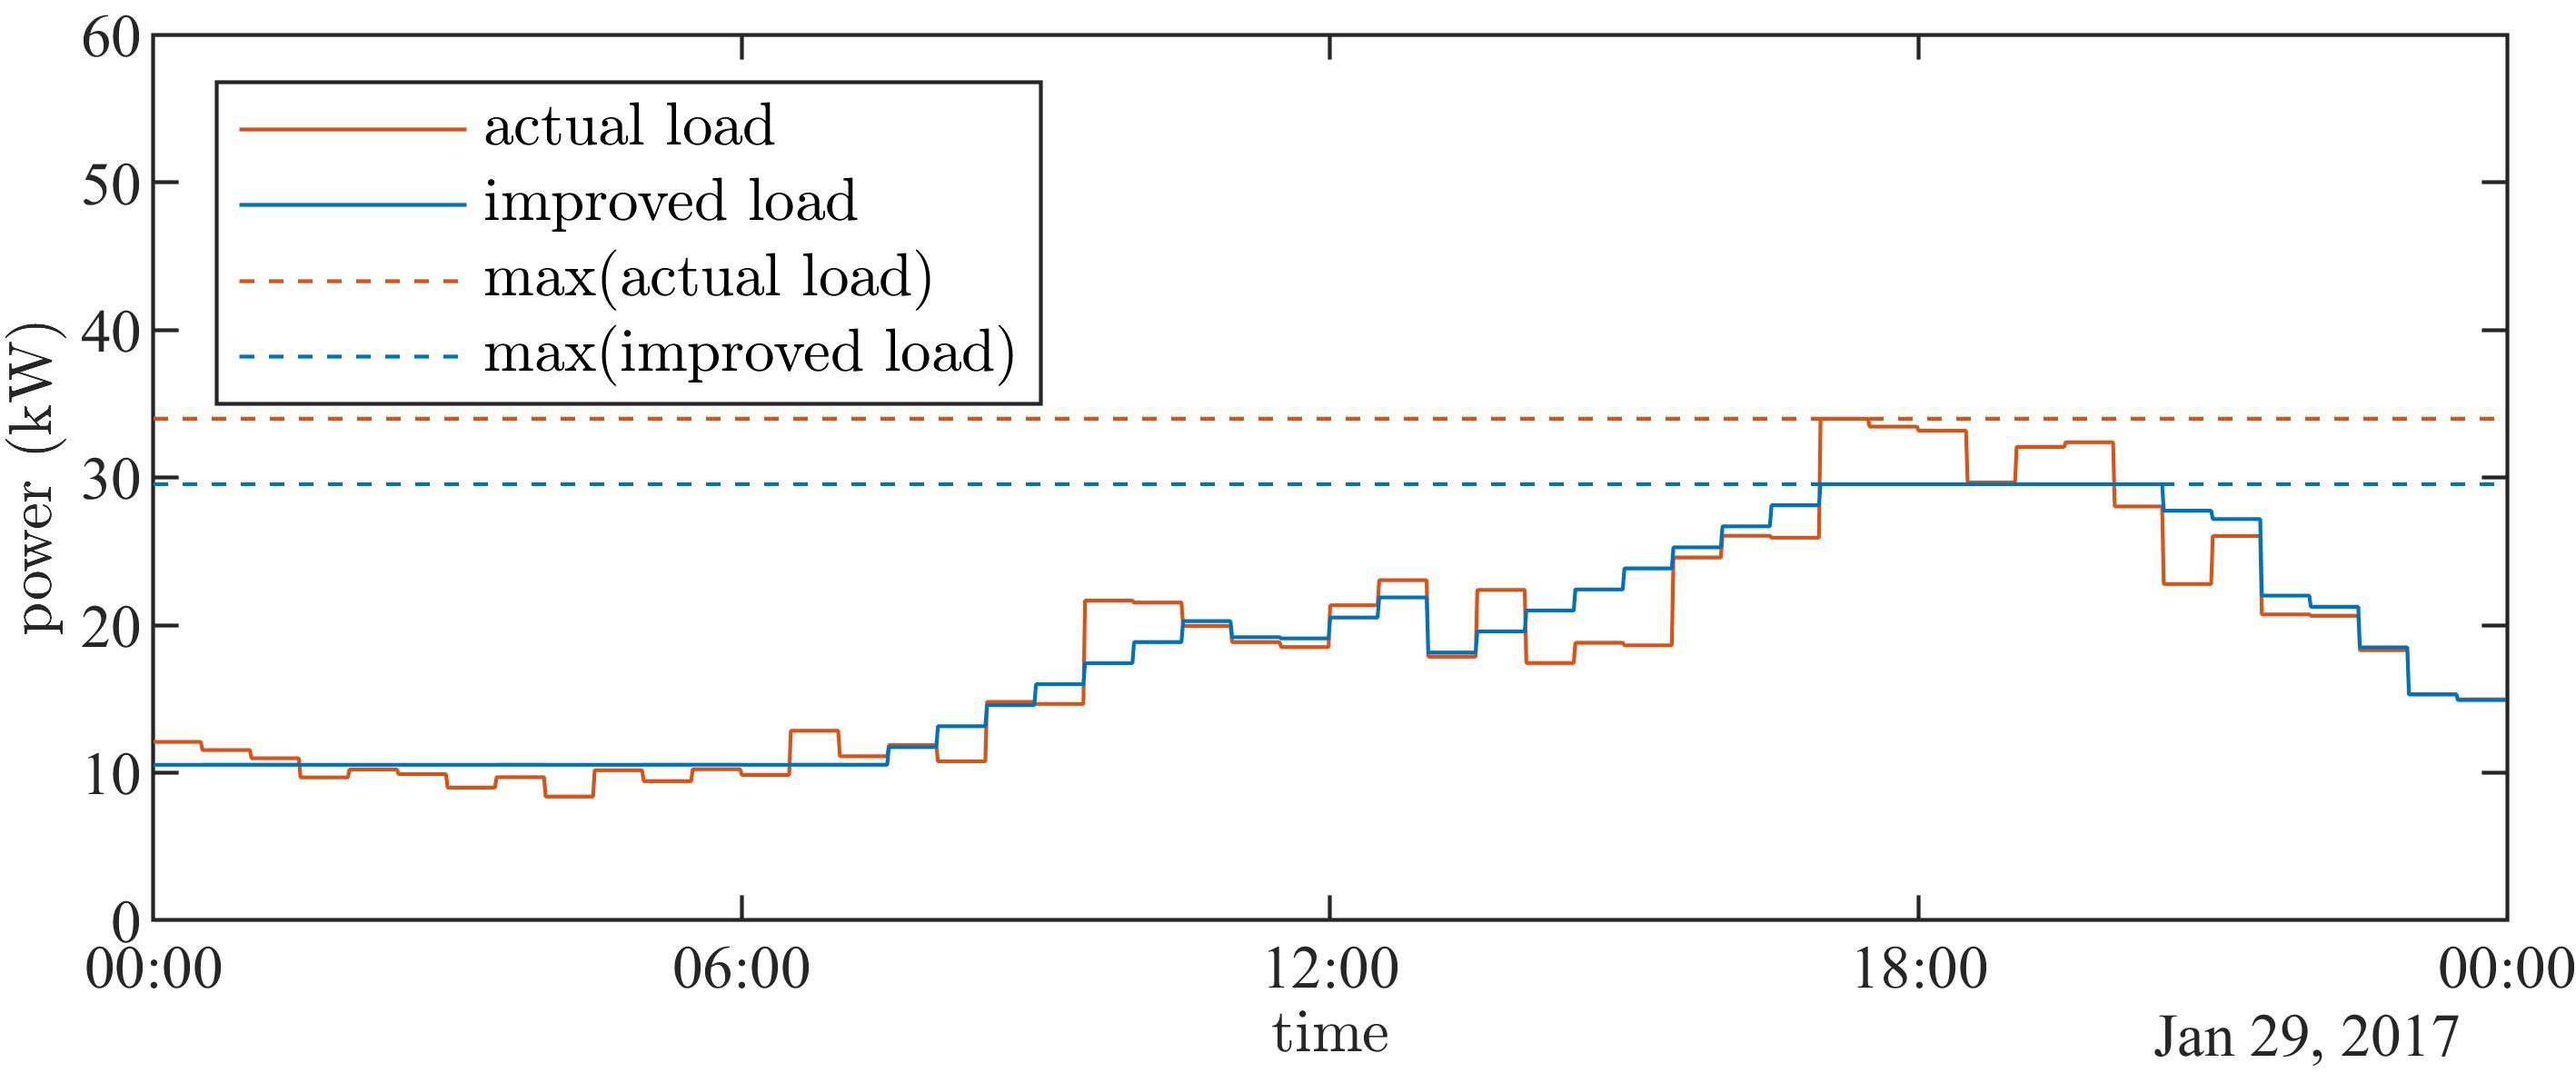
\includegraphics{_chapter2/fig/day-forecasted}
		\label{ch2:subfig:day-forecasted}
	}\\
	\subfloat[]{%
		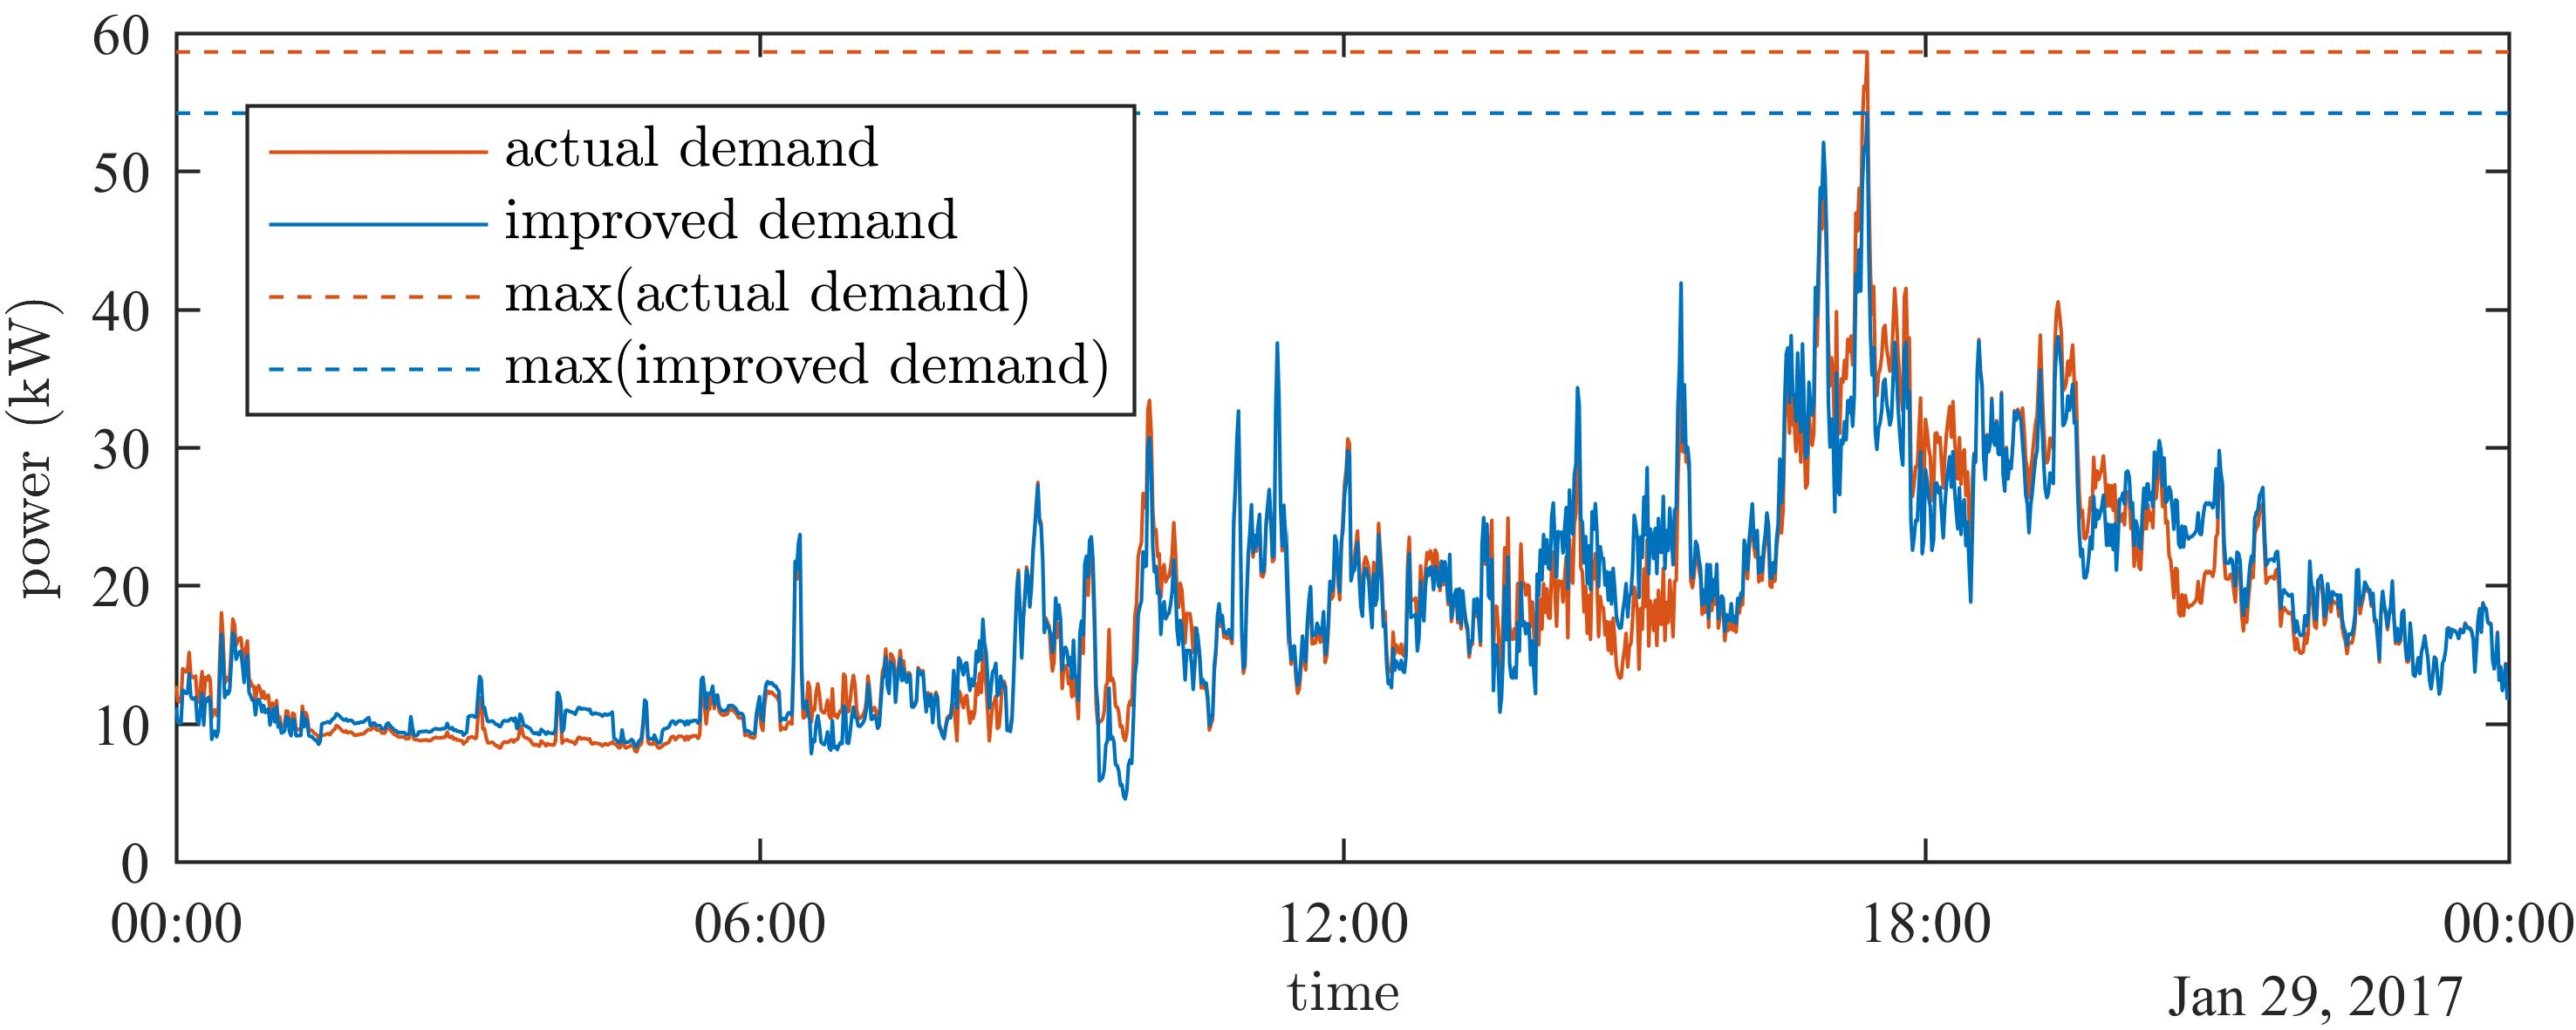
\includegraphics{_chapter2/fig/day-actual}
		\label{ch2:subfig:actual-forecasted}
	}
	\caption{An example of applying a half-hourly ESMU schedule to \hl{the half-hourly substation load} (Subfig. \ref{ch2:subfig:day-forecasted}) and the actual, sub-half-hourly daily load\hl{, measured at the substation} (Subfig. \ref{ch2:subfig:actual-forecasted}).}
	\label{ch2:fig:cost-sample}
\end{figure}